% !TEX root = ../main.tex
% Chapter 1
\chapter{Introduction}

\label{Chapter1} % For referencing the chapter elsewhere, use~\ref{Chapter1}

\lhead{Chapter 1. \emph{Introduction}} % This is for the header on each page - perhaps a shortened title

With the wide availability of smartphones and built-in inertial sensors, more and more applications of \gls{har} are introduced \cite{avci2010activity,derawi2010accelerometer,guenterberg2009distributed}.
Many approaches to recognize the performed activity rely on classification of recorded data \cite{devaul2001real,ward2006activity,yang2008using,anguita2012human,bao2004activity,bernecker2012activity,he2008activity}, which can be done online or in batches after the performance \cite{duque2012offline}.
Often time windows are used, which form short consecutive segments of data and are processed in a model construction and recognition phase.
The constructed model is used to determine which (earlier learned) activity is performed.
Besides the explicit classification of the data, an implicit obtained result is a segmentation of performed activities over time.

The goal of this thesis is to create an method for online temporal segmentation of time series data.
This will be performed explicitly, prior to the classification of data segments to learned activities.

Our assumption is that a temporal segmentation of time series can be beneficial information for classification methods.
Instead of using a fixed window approach, the classification methods can use a larger set of homogeneous data.
Thereby, the methods have more information to create a solid model of the activities.

To find a temporal segmentation, we rely on change detection in time series.
In the context of this research the time series consists of recordings from inertial sensors during the performance of human activities.
The sensors, such as the accelerometer, are nowadays widely available in smartphones.
We are interested in real-world data from both in- and outdoor activities performed in a continuous manner.

Compared to recordings in a controlled laboratory environment, we expect the real-world data to be prone to unexpected characteristics.
The constructed method must be robust in order to handle these.

For the change detection algorithm we will use a special form of a \gls{svm}, the \gls{occ} based \gls{svdd}, as introduced by Tax~\cite{tax2001one}.
This method models the data in the shape of a high-dimensional hypersphere.
From this hypersphere the radius is extracted, which can be used as an indication of change and be processed by one-dimensional change detection algorithms.
The radius of the hypersphere is used in the following relation.
When the performed activity changes, so will the data distribution and characteristics.
This results in a change of the constructed model, especially in the radius of the hypersphere.
Thus, a change in the radius indicates a changes in the performed activity.

The remainder of this introduction is organized as follows.
In \Cref{sec:intro_scope} the scope of this thesis is discussed.
A short discussing on the workings of an \acrlong{oc-svm} is provided in \Cref{sec:intro_ocsvm}.
The data sets we have used in this work are discussed in \Cref{sec:intro_data_sets}.
\Cref{sec:intro_contributions} gives a short overview of our contributions.
Finally, \Cref{sec:intro_thesis_structure} outlines the structure of this thesis.

\section{Scope}\label{sec:intro_scope}
The scope of this thesis are segmentation methods of inertial sensor data in the field of machine learning.
The type of data is inertial sensor time series, collected by on-body worn sensors as found in smartphones.
These time series are recorded during the performance of real-world human activities.
The setting of the activities are real-world environments, both in- and outdoor.

As mentioned in the previous section, a segmentation is often obtained as a by-product from direct windowed classification.
Other approaches have a very rigid form of segmentation, \eg by limiting the number of possible segment types \cite{himberg2001time,chamroukhi2013joint}, or have applied it to different type of time series data.
In Fuchs \etal \cite{fuchs2010online} artificial sinusoidal data is processed.
Li and Zheng \cite{li2007segmentation} use visual motion data streams to find patterns of activities.
The method of Guenterberg \etal \cite{guenterberg2009automatic} is able to distinguish periods of rest and activity in inertial sensor data streams.
Others have extracted features from windows of data which are used for the segmentation \cite{guo2012adaptive}.
These activities include sitting, standing, walking, running, and ascending and descending staircases.

The problem of finding a temporal segmentation can be seen as a sub-problem to the problem of Activity Classification.
This relation is illustrated in \Cref{fig:thesis_goal}.
The figure visualizes that we can apply classification on time series data.
In many approaches it is applied to (partially overlapping) windows of data.
In the context of \gls{har}, the window length commonly consists of around two seconds of data.
In our setup we perform temporal segmentation, instead of using a fixed window length.
Each segment will consist of homogeneous data, in the sense that the underlying data generating activity should not change within a segment.
Likewise, the previous and next segments (if present) should be generated by a different activity.

\begin{figure}[h]
  \centering
    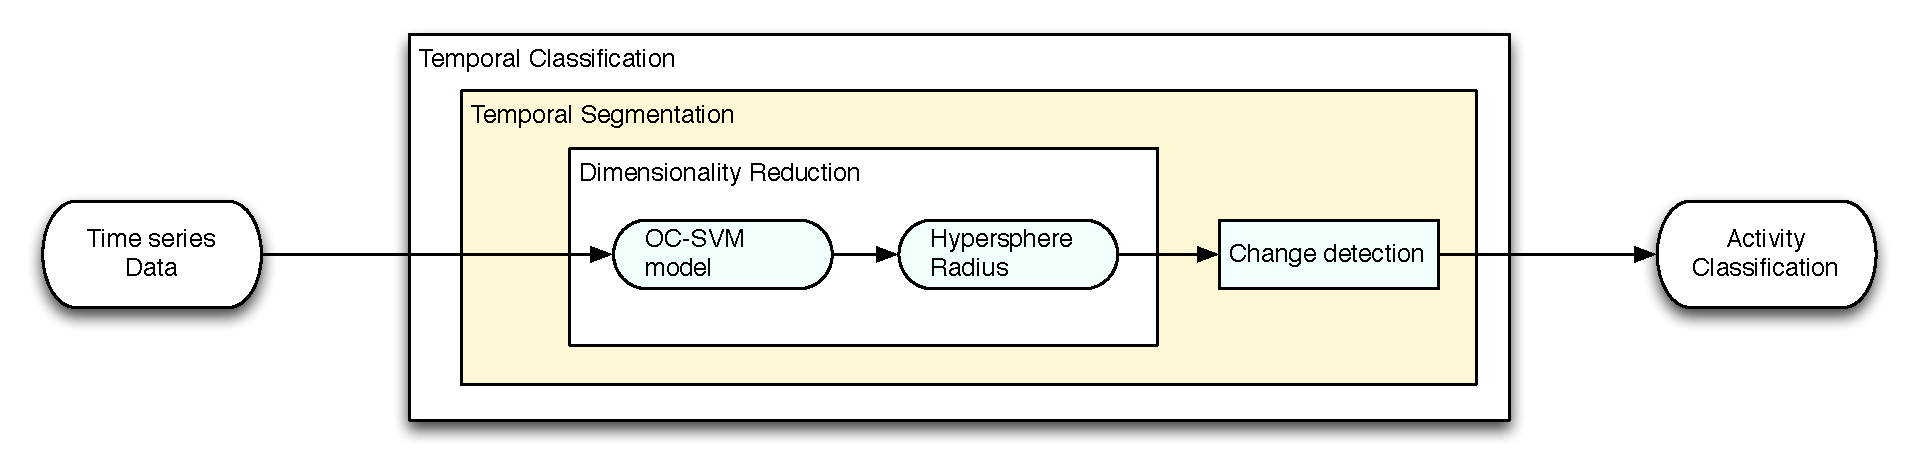
\includegraphics[width=\textwidth,height=\textheight,keepaspectratio]{./Figures/chapter1/thesis_goal.pdf}
  \caption[Thesis goal]{The goal of this thesis. The scope of this thesis is Temporal Segmentation, which can be useful in the context of Temporal Classification. Given a data set, we construct a \gls{oc-svm} high-dimensional spherical model, from which we extract the radius. This metric is then applied to direct change detection algorithms. The detected change points can support the classification of homogeneous segments of data.}
  \label{fig:thesis_goal}
\end{figure}

To find these segments of homogeneous data, we employ a model construction phase.
The \acrlong{oc-svm} transforms the data to a higher dimensional space.
Non-linear mapping functions are used to add flexibility to the classification decision boundary.
In the higher dimensional space an enclosing boundary around the data points, in the shape of a hypersphere, is constructed.
The size, expressed as the radius, of the hypersphere depends on the distribution of the data points in the model.
We will use the radius of this hypersphere as a characterizing metric and base our change detection on it.

The model processes the data in windows of fixed length.
A change in data distribution and characteristics should then result in a change of the hypersphere's radius.
Such a (sudden) change in the radius thus reflects a change in the time series data.
It indicates the end of the current and the beginning of a new segment.
In \Cref{sec:literature_review_temporal_segmentation} a detailed overview of temporal segmentation methods is given.
Information about segments can be used in the classification phase of \gls{har}.
Instead of using relatively small windows, it can apply classification to the full segments of data.
The final result, which is outside the scope is this thesis, will be a full classification of activities over the time series data.

\section{One-Class Support Vector Machines}\label{sec:intro_ocsvm}
In the setup, as described in the previous section and visualized in \Cref{fig:thesis_goal}, we employ a model construction phase.
For this model we will use an \acrlong{oc-svm} implementation: the \acrlong{svdd} algorithm by Tax~\cite{tax2001one}.
In earlier research multi-class \glspl{svm} are used for direct classification of inertial sensor data \cite{he2008activity,mountrakis2011support,anguita2012human}.
Others have used \gls{oc-svm} classifiers for novelty or outlier detection \cite{scholkopf1999support,camci2010change,li2003improving,ma2003time,tax1999support}.
The method by Yin \etal  \cite{yin2008sensor} creates a \gls{oc-svm} classifier to filter normal activity traces, using training data.
However, to the best of our knowledge, \gls{oc-svm} methods have not yet been applied to inertial sensor time series data directly to find changes in behavior and create a temporal segmentation.

The \glspl{oc-svm} algorithms transforms the time series data, which can be of any high dimension, to a higher dimensional feature space.
When the data is assumed to be of the same class, it can be characterized by an enclosing boundary.
In case of the \gls{svdd} algorithm this boundary is in the shape of a hypersphere.
Using this model, we are able to test the membership of a new data point to the described class.
The new data point is transformed to the feature space and its location is compared to the boundary.
If it lies within the boundary then it is a member of the class and otherwise it is regarded as an outlier.

In case the data distribution changes, the data points will have a larger variance.
It will result in a larger hypersphere in the feature space.
This means that a change in the underlying process of a time series data results in a larger hypersphere radius.
Thus the \gls{oc-svm} method allows us to reduce a complex high-dimensional signal to an one-dimensional time series data.
The reduced time series can be inspected by simpler change detection methods, in a number of ways.
\Cref{Chapter3} will discuss the \gls{oc-svm} methods in detail and \Cref{Chapter4} elaborates on the overall change detection method.

\section{Data sets}\label{sec:intro_data_sets}
In recent research two data sets for \gls{har} have been made public.
In order to benchmark our proposed method we applied our method to these data sets.
However, it turned out the data sets were not appropriate for continuous temporal segmentation.
In the \gls{wisdm} set \cite{kwapisz2011activity} the activities are not performed continuously.
There is no transition period between activities.
Since we are interested in the detection changes between consecutive activities, we can not use this data set.
The \gls{uci-har} from \cite{anguita2012human} also lacks continuous recordings.
Furthermore, it seems to have incorrect labels.
Finally, for both data sets there are no visual images of the performed activities.
So in case of ambiguity there is no ground truth to consult.
To overcome these problems, we have created our own real-world data set: \acrlong{almende-data} \cite{vlasveld2014acras}.

Our own data set is recorded by placing a smartphone with inertial sensors in the front right pants pocket of a subject.
The subject was asked to perform common and simple activities in a natural environment, both in- and outdoors.
During the performance the subjects were also recorded with a video camera from a third-person point of view.
This allows us to create a ground truth for the temporal segmentation of performed activities.

Besides the recorded data sets we have used artificial data sets to obtain an objective, quantitative, performance measure of the method.
These artificial data sets are modeled to the sets used in \cite{camci2010change,takeuchi2006unifying}.
In \Cref{Chapter5} we discuss the artificial data sets and results in detail.
The real-world recordings and results are discussed in \Cref{Chapter6}.

\section{Contributions}\label{sec:intro_contributions}
As a result from our proposed method and application to recorded real-world data sets, this thesis will provide the following contributions:
\begin{enumerate}
  \item \textbf{Continuous recorded human activity data:} the proposed method is applied to our own recorded human activity data.
  This data set can be grounded by using the video recordings of the subject while performing the activities.
  The data set, consisting of raw inertial sensor recordings, manual change point and activity labeling, and video recordings, is used for testing the method and is made available to the public \cite{vlasveld2014acras}.
  \item \textbf{Application of \gls{oc-svm} methods to inertial sensor data:} to the best of our knowledge, this thesis is the first application of \gls{oc-svm} methods, especially the \gls{svdd} method, to inertial sensor signals in the context of temporal segmentation.
  Furthermore, this thesis contributes to research that has temporal segmentation of inertial sensor data as its primary objective.
  \item \textbf{Adaptation of \acrshort{svcpd}:} we have adopted and simplified the \acrshort{svcpd} method by Camci~\cite{camci2010change} in order to find change points in time series data.
  In our simplification we have not encountered a noticeably decrease in performance.
\end{enumerate}

\section{Thesis structure}\label{sec:intro_thesis_structure}
The structure of this thesis is as follows.
In \Cref{Chapter2} a literature review is provided.
We will look at the different interpretations and implementations for change, novelty, and outlier detection.
Previous work in the field of \gls{har} is discussed and we end with existing applications of \glspl{svm} to change detection.
\Cref{Chapter3} further analyses \glspl{svm} and two implementations of \glspl{oc-svm}.
It relates the properties of the constructed \gls{oc-svm} models to change detection in time series data.
That relation is applied to our problem formulation in \Cref{Chapter4}, where we construct our change detection method \gls{ocs-hats}~\cite{vlasveld2014hats}, based on the work of Camci~\cite{camci2010change}.
In \Cref{Chapter5} we apply the method to artificial data and show the quantitative performance.
In \Cref{Chapter6} the method is applied to our real-world \gls{almende-data} \cite{vlasveld2014acras}.
In that chapter we show, by qualitative analysis, the ability of detecting change in \gls{har} data, recorded by inertial sensors.
This thesis is concluded in \Cref{Chapter7}, in which we reflect on the performed research and state possibilities for feature research.